% This is "sig-alternate.tex" V2.1 April 2013
% This file should be compiled with V2.5 of "sig-alternate.cls" May 2012
%
% This example file demonstrates the use of the 'sig-alternate.cls'
% V2.5 LaTeX2e document class file. It is for those submitting
% articles to ACM Conference Proceedings WHO DO NOT WISH TO
% STRICTLY ADHERE TO THE SIGS (PUBS-BOARD-ENDORSED) STYLE.
% The 'sig-alternate.cls' file will produce a similar-looking,
% albeit, 'tighter' paper resulting in, invariably, fewer pages.
%
% ----------------------------------------------------------------------------------------------------------------
% This .tex file (and associated .cls V2.5) produces:
%       1) The Permission Statement
%       2) The Conference (location) Info information
%       3) The Copyright Line with ACM data
%       4) NO page numbers
%
% as against the acm_proc_article-sp.cls file which
% DOES NOT produce 1) thru' 3) above.
%
% Using 'sig-alternate.cls' you have control, however, from within
% the source .tex file, over both the CopyrightYear
% (defaulted to 200X) and the ACM Copyright Data
% (defaulted to X-XXXXX-XX-X/XX/XX).
% e.g.
% \CopyrightYear{2007} will cause 2007 to appear in the copyright line.
% \crdata{0-12345-67-8/90/12} will cause 0-12345-67-8/90/12 to appear in the copyright line.
%
% ---------------------------------------------------------------------------------------------------------------
% This .tex source is an example which *does* use
% the .bib file (from which the .bbl file % is produced).
% REMEMBER HOWEVER: After having produced the .bbl file,
% and prior to final submission, you *NEED* to 'insert'
% your .bbl file into your source .tex file so as to provide
% ONE 'self-contained' source file.
%
% ================= IF YOU HAVE QUESTIONS =======================
% Questions regarding the SIGS styles, SIGS policies and
% procedures, Conferences etc. should be sent to
% Adrienne Griscti (griscti@acm.org)
%
% Technical questions _only_ to
% Gerald Murray (murray@hq.acm.org)
% ===============================================================
%
% For tracking purposes - this is V2.0 - May 2012

\documentclass{sig-alternate-05-2015}
\usepackage{multirow}
\usepackage{xcolor}
\usepackage{caption}
\usepackage{float}

\newcommand{\rk}[1]{\textcolor{blue}{#1}}


\begin{document}

% Copyright
\setcopyright{acmcopyright}
%\setcopyright{acmlicensed}
%\setcopyright{rightsretained}
%\setcopyright{usgov}
%\setcopyright{usgovmixed}
%\setcopyright{cagov}
%\setcopyright{cagovmixed}


% DOI
\doi{10.475/123_4}

% ISBN
\isbn{123-4567-24-567/08/06}

%Conference
\conferenceinfo{PLDI '13}{June 16--19, 2013, Seattle, WA, USA}

\acmPrice{\$15.00}

%
% --- Author Metadata here ---
\conferenceinfo{WOODSTOCK}{'97 El Paso, Texas USA}
%\CopyrightYear{2007} % Allows default copyright year (20XX) to be over-ridden - IF NEED BE.
%\crdata{0-12345-67-8/90/01}  % Allows default copyright data (0-89791-88-6/97/05) to be over-ridden - IF NEED BE.
% --- End of Author Metadata ---
\title{Stochastic Block Models with Multiple Continuous Attributes}
%\title{Alternate {\ttlit ACM} SIG Proceedings Paper in LaTeX
%Format\titlenote{(Produces the permission block, and
%copyright information). For use with
%SIG-ALTERNATE.CLS. Supported by ACM.}}
%\subtitle{[Extended Abstract]
%\titlenote{A full version of this paper is available as
%\textit{Author's Guide to Preparing ACM SIG Proceedings Using
%\LaTeX$2_\epsilon$\ and BibTeX} at
%\texttt{www.acm.org/eaddress.htm}}}
%
% You need the command \numberofauthors to handle the 'placement
% and alignment' of the authors beneath the title.
%
% For aesthetic reasons, we recommend 'three authors at a time'
% i.e. three 'name/affiliation blocks' be placed beneath the title.
%
% NOTE: You are NOT restricted in how many 'rows' of
% "name/affiliations" may appear. We just ask that you restrict
% the number of 'columns' to three.
%
% Because of the available 'opening page real-estate'
% we ask you to refrain from putting more than six authors
% (two rows with three columns) beneath the article title.
% More than six makes the first-page appear very cluttered indeed.
%
% Use the \alignauthor commands to handle the names
% and affiliations for an 'aesthetic maximum' of six authors.
% Add names, affiliations, addresses for
% the seventh etc. author(s) as the argument for the
% \additionalauthors command.
% These 'additional authors' will be output/set for you
% without further effort on your part as the last section in
% the body of your article BEFORE References or any Appendices.

\numberofauthors{4} %  in this sample file, there are a *total*
% of EIGHT authors. SIX appear on the 'first-page' (for formatting
% reasons) and the remaining two appear in the \additionalauthors section.
%
\author{
% You can go ahead and credit any number of authors here,
% e.g. one 'row of three' or two rows (consisting of one row of three
% and a second row of one, two or three).
%
% The command \alignauthor (no curly braces needed) should
% precede each author name, affiliation/snail-mail address and
% e-mail address. Additionally, tag each line of
% affiliation/address with \affaddr, and tag the
% e-mail address with \email.
%
% 1st. author
Natalie Stanley, Thomas Bonacci, Roland Kwitt, Marc Niethammer, Peter J. Mucha
%\alignauthor
%Natalie Stanley\\
%       \affaddr{University of North Carolina, Chapel Hill}\\
%       %\email{stanleyn@email.unc.edu}
%   \alignauthor
%Thomas Bonacci\\
%\affaddr{University of North Carolina, Chapel Hill}
%%\email{thomas.bonacci@gmail.com}
%% 2nd. author
%\alignauthor
%Roland Kwitt\\
%	\affaddr{University of Salzburg}
%      % \email{Roland.Kwitt@sbg.ac.at}
%% 3rd. author
%\alignauthor Marc Niethammer\\
%       \affaddr{University of North Carolina, Chapel Hill}\\
%       %\email{mn@cs.unc.edu}
%\and  % use '\and' if you need 'another row' of author names
%% 4th. author
%\alignauthor Peter J. Mucha\\
%       \affaddr{University of North Carolina, Chapel Hill}\\
       % \email{mucha@unc.edu}
% 5th. author
%\alignauthor Sean Fogarty\\
%       \affaddr{NASA Ames Research Center}\\
%       \affaddr{Moffett Field}\\
%       \affaddr{California 94035}\\
%       \email{fogartys@amesres.org}
%% 6th. author
%\alignauthor Charles Palmer\\
%       \affaddr{Palmer Research Laboratories}\\
%       \affaddr{8600 Datapoint Drive}\\
%       \affaddr{San Antonio, Texas 78229}\\
%       \email{cpalmer@prl.com}
}
% There's nothing stopping you putting the seventh, eighth, etc.
% author on the opening page (as the 'third row') but we ask,
% for aesthetic reasons that you place these 'additional authors'
% in the \additional authors block, viz.
%\additionalauthors{Additional authors: John Smith (The Th{\o}rv{\"a}ld Group,
%email: {\texttt{jsmith@affiliation.org}}) and Julius P.~Kumquat
%(The Kumquat Consortium, email: {\texttt{jpkumquat@consortium.net}}).}
%\date{30 July 1999}
% Just remember to make sure that the TOTAL number of authors
% is the number that will appear on the first page PLUS the
% number that will appear in the \additionalauthors section.

\maketitle
\begin{abstract}
Stochastic block models (SBMs) are probabilistic models for community structure in networks in which nodes within a community are assumed to be connected to nodes within and between communities in a uniform, characteristic way.  Typically, only the adjacency matrix is used to perform SBM parameter inference. In this paper, we consider circumstances in which nodes have an associated vector of continuous attributes. The model assumes that the attributes associated with nodes in a network's community can be described by a particular multivariate Gaussian model. Moreover, in this augmented SBM, the objective is to learn the SBM and multivariate gaussian parameters describing each community. While there are recent examples in the literature that combine connectivity and attribute information, we are to our knowledge the first to consider the effect of multiple continuous attributes. We highlight the usefulness of our model for two two network prediction tasks: collaborative filtering and link prediction. As a result of fitting this attributed stochastic block model, one can predict the attribute vector or connectivity patterns for a new node in the event of the complementary source of information (connectivity or attributes, respectively). While our approach is the first stochastic block model (to our knowledge) to include multiple continuous attributes, we highlight the ability of our approach in two tasks: link prediction in collaborative filtering. In this work, we demonstrate the usefulness of our model in two different types of biological networks. 

First, we consider a network between a set of subjects encoding the similarity in the bacterial species counts in their microbiomes. For each subject, we consider attributes, such as, BMI, nationality, and age. Second, We consider a protein interaction network encoding regulatory relationships, augmented with experimental data about function and abundance. 

Data for tasks 1 and 2:
\url{https://www.nature.com/articles/ncomms5344}
 \url{http://pubs.acs.org/doi/full/10.1021/pr401258d}
\end{abstract}



%In collaborative filtering, one seeks to predict an attribute of a node, based on the attributes of its neighbors. With our fitted attributed SBM, this task becomes simple and can  We demonstrate our approach on two biological datasets. First, we consider a similarity network of between subjects' microbial species abundances in a microbiome analysis, with attributes being the probability of belonging to 1 of 6 body mass index classifications. Second, we consider a protein interaction network, where the attributes are characteristics of the protein. 



%
% The code below should be generated by the tool at
% http://dl.acm.org/ccs.cfm
% Please copy and paste the code instead of the example below. 
%
%\begin{CCSXML}
%<ccs2012>
% <concept>
%  <concept_id>10010520.10010553.10010562</concept_id>
%  <concept_desc>Computer systems organization~Embedded systems</concept_desc>
%  <concept_significance>500</concept_significance>
% </concept>
% <concept>
%  <concept_id>10010520.10010575.10010755</concept_id>
%  <concept_desc>Computer systems organization~Redundancy</concept_desc>
%  <concept_significance>300</concept_significance>
% </concept>
% <concept>
%  <concept_id>10010520.10010553.10010554</concept_id>
%  <concept_desc>Computer systems organization~Robotics</concept_desc>
%  <concept_significance>100</concept_significance>
% </concept>
% <concept>
%  <concept_id>10003033.10003083.10003095</concept_id>
%  <concept_desc>Networks~Network reliability</concept_desc>
%  <concept_significance>100</concept_significance>
% </concept>
%</ccs2012>  
%\end{CCSXML}

%\ccsdesc[500]{Computer systems organization~Embedded systems}
%\ccsdesc[300]{Computer systems organization~Redundancy}
%\ccsdesc{Computer systems organization~Robotics}
%\ccsdesc[100]{Networks~Network reliability}


%
% End generated code
%

%
%  Use this command to print the description
%
\printccsdesc

% We no longer use \terms command
%\terms{Theory}

\keywords{Stochastic Block Model, Networks, Community Detection, Attributes, Image Analysis}

\section{Introduction}
\subsection{Network data and node attributes}
Uncovering patterns in network data is a common pursuit across a range of fields, such as in biology \cite{dan}, medicine \cite{cancer} and computational social science \cite{socialnetwork}. A powerful way to analyze mesoscale structural organization within a network is with community structure \cite{muchacommunity,jurecommunity}. In this pursuit, the objective is to identify cohesive groups of nodes with a high density of within-group connections and few between-group connections. Numerous approaches exist to accomplish this task \cite{muchacommunity,jurecommunity}, but typically only the adjacency matrix conveying the wiring of the graph is taken into account. In certain applications, each node in a network is equipped with additional information (or particular attributes) that was not implicitly taken into account in the construction of the network. For example, one could consider a collection of attributes measured for individuals in a social network (i.e., age, income, level of education). In this work, we seek to incorporate these attributes in the community detection task, such that communities are able to effectively combine both sources of information to understand the organization of components in a system.

\vskip2ex
\indent Further motivation for the incorporation of node attributes in community detection is also inspired by detectability of communities, as well as possible impact in the image analysis community. The detectability limit in networks is a theoretical notion of the relationship between the number of within-community connections to the number of between-community connections that allows for algorithms to accurately detect community structure \cite{newmanDetect,mooreDetect}. In circumstances where the number of within-community connections is sparse, we propose that the incorporation of attribute information will make communities easier to detect. Further, graph-based image segmentation has shown promise \cite{malikSeg,browetCommunity}, however the probabilistic notion of communities in this context is not well explored. 

\subsection{Related work}
The incorporation of node attributes in network analysis tasks is not well explored, particularly in the context of probabilistic network models. In a modularity based approach, the authors of \cite{ilouvain} modified the classical modularity quality function to incorporate node attribute information. Two probabilistic network and attribute models have also been proposed by \cite{cesna,clauset}. In \cite{cesna}, the authors developed a generative model for attributed network data based on node affiliation. However, in this approach only binary attribute data are considered. In \cite{clauset}, the authors developed a probabilistic framework for incorporating metadata or attributes in community detection, however, the model takes \rk{only a single metadata 
value for each node into account}. We seek to extend these existing approaches to reflect continuous attribute data and particularly multidimensional attribute data drawn from a multivariate Gaussian distribution. 

New stuff to add: peel, clauset controversy, tiago and dhric

\subsection{Stochastic Block Models}
To accomplish our objective of integrating node attributes in a probabilistic framework, we will \rk{model} connectivity in a network with the widely-used stochastic block model \rk{(SBM)} \cite{hollandSBM}. This model assumes that edges within a community are connected within and between communities in a characteristic or probabilistic way. To fit this model to network data, the objective is to partition the nodes into communities, such that these assignments maximize the likelihood of the model according to the observed edges. In this inference problem for a network with $N$ nodes and $K$ communities, a $K \times K$ probability matrix, ${\bf theta}$ and a $N$-length vector, ${\bf z}$ are learned. The matrx ${\theta}$ described the probability of connections within and between communities, while ${\bf z}$ gives the node-to-community assignments. While this modeling framework is well-studied, recent attention hs focused on the ability to integrate extra information (attributes or metadata), into the inference problem and whether it is appropriate to do so. 

\subsection{Contributions and Paper Outline}
We summarize our contributions to the problem of finding communities in attributed network data as follows.
\begin{itemize}
\item We developed a probabilistic model for node-to-community structure that uses adjacency matrix connectivity and continuous node attributes to determine a community assignment for the nodes. Our model is the first to our knowledge to allow for the augmentation of a classic stochastic block model with multiple continuous attributes. 
\item We provide details for the inference technique that can be used to effectively estimate model parameters.
\item We demonstrate that by fitting an attributed stochastic block model allows for good performance in link prediction and collaborative filtering results. In particular, we demonstrate these tasks on two different biological examples. 
\end{itemize}

The paper is organized as follows. In section 2, we describe the model and inference methods for estimating parameters. In section 3, we perform experiments on synthetic networks. Section 4 shows how the method can be applied in image segmentation tasks. Finally in section 5 we discuss the method, its limitations and future work. 

\section{Model}
\subsection{Objective}
We seek to incorporate both connectivity (${\bf A}$) and attribute information (${\bf X}$) to infer node-to-community assignments, ${\bf Z}$. Note that for a network with $N$ nodes, \rk{$K$} communities and $p$ measured attributes, ${\bf A}$, ${\bf X}$, and ${\bf Z}$ have dimensions $N \times N$, $N \times p$ and $N \times K$, respectively. In particular, ${\bf Z}$ is a binary indicator matrix, where entry $z_{ic}$ is 1 if and only if node $i$ belongs to community $c$. We also define ${\bf z}$ to be the \rk{$N$-dimensional} vector of node-to-community assignments. Following the assumption of \cite{cesna}, we assume that connectivity and attributes are conditionally independent, given the community membership label. The graphical model for the relationship between node-to-community labels, connectivity and attribute information is shown in Fig.~\ref{fig:graphical_model}.

\begin{figure}
\begin{center}
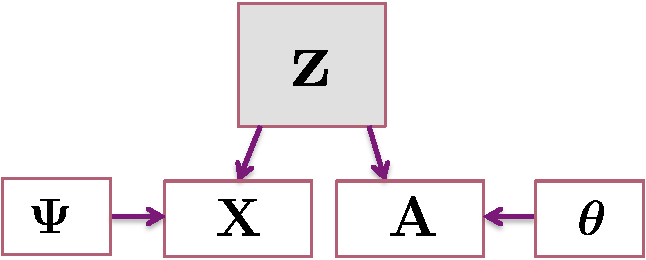
\includegraphics[scale=0.5]{GraphModel.pdf}
\caption{{\bf Modeling community membership in terms of attributes and connectivity}. Node-to-community assignments specified by ${\bf z}$ are determined in terms of adjacency matrix information, ${\bf A}$ and attribute matrix information, ${\bf A}$. ${\bf A}$ and ${\bf X}$ are assumed by be generated from a stochastic block model and a mixture of multivariate gaussian distributions, parameterized by ${\boldsymbol \theta}$ and ${\boldsymbol \Psi}$, respectively.
\label{fig:graphical_model}} 
\end{center}
\end{figure}

To infer the ${\bf Z}$ that best explains the data, we adopt a likelihood maximization approach. That is, we seek to find the partition of nodes to communities that best \rk{describes} the observed connectivity and attribute information.  Given the conditional independence assumption of ${\bf X}$ and ${\bf A}$, we can express the log likelihood of the data, ${\mathcal L}$ as the sum of connectivity and attribute log likelihoods, ${\mathcal L}_{A}$ and ${\mathcal L}_{X}$, respectively,
as
\begin{equation}
\mathcal{L}=\mathcal{L}_{A}+\mathcal{L}_{X}\enspace.
\label{eqn:likelihood_decomposition}
\end{equation}

This likelihood reflects the joint distribution of the adjacency matrix, ${\bf A}$, the attribute matrix, ${\bf X}$, and the matrix of node-to-community indicators, ${\bf Z}$; formally, we have 

\begin{equation}
\mathcal{L}=p({\bf A},{\bf X},{\bf Z})\enspace. 
\end{equation}

Given that ${\bf Z}$ is a latent variable that we are trying to infer, we can approach the problem using the expectation maximization (EM) algorithm \cite{EM}. By doing this, we will alternate between estimating the posterior probability that a node $i$ has community label $c$, or

\begin{equation}
\label{post}
p(z_{ic}=1\mid {\bf X,A})
\end{equation} 
and estimates for ${\boldsymbol \theta, \boldsymbol \Psi}$, i.e., the model parameters specifying the adjacency and attribute matrices, respectively. 

\subsection{Attribute Likelihood}

For a network with $K$ communities, we assume that each particular community $i$ \rk{has an associated} $p$-dimensional mean ${\boldsymbol \mu}_{i}$ and $p \times p$ covariance matrix, ${\boldsymbol \Sigma}_{i}$. Note that these parameters \rk{uniquely identify} a $p$-dimensional multivariate Gaussian distribution. To specify this model for all $K$ communities, we define the parameter ${\boldsymbol \Psi}=\{{\boldsymbol \mu}_{1},{\boldsymbol \mu}_{2},\dots {\boldsymbol \mu}_{k},{\boldsymbol \Sigma}_{1},{\boldsymbol \Sigma}_{2},\dots {\boldsymbol \Sigma}_{K}\}$. Then, \rk{the} probability of the $i$-th row of ${\bf X}$, \rk{denoted as} ${\bf x}_{i}$, giving the values of the $p$ attributes for node $i$, can be modeled as

\begin{equation}
p({\bf x}_{i} \mid {\boldsymbol \Psi})=\sum_{c=1}^{K}\pi_{c}p({\bf x}_{i} \mid {\boldsymbol \mu}_{c},{\boldsymbol \Sigma}_{c})\enspace.
\end{equation}

Here, $p({\bf x}_{i} \mid {\boldsymbol \mu}_{c},{\boldsymbol \Sigma}_{c})$ is the probability density function for the multivariate Gaussian and $\pi_{c}$ is the probability that a node is assigned to community $c$.

\subsection{Adjacency Matrix Likelihood}
For the adjacency matrix, ${\bf A}$ and the $K \times K$ matrix of stochastic block model parameters, ${\boldsymbol \theta}$, the probability of observing the connectivity pattern of node $i$, or the $i$-th row in the adjacency matrix, \rk{denoted as} ${\bf a}_{i}$, is given by

\begin{equation}
\begin{split}
\log p({\bf a}_{i} \mid {\boldsymbol{Z}},{\boldsymbol \theta})&=\sum_{c_{1}=1}^{k}z_{i,c_{1}}[\sum_{c_{2}=1}^{k}\sum_{j \in \mathcal{N}(i)}z_{j,c_{2}}\log({\boldsymbol \theta}_{c_{1},c_{2}}) \\
&-\sum_{j \notin \mathcal{N}(i)}z_{j,c_{2}}\log(1-{\boldsymbol \theta}_{c_{1},c_{2}})]
\end{split}
\end{equation}

\subsection{Inference}
To use EM to maximize the likelihood of the data, we break the process into the E-step and M-Step.

\rk{\textbf{E-Step.}} During the E-step, we use the current value of learned model parameters, ${\boldsymbol \theta}$ and ${\boldsymbol \Psi}$ to compute the posterior, given in Eq.~\eqref{post}. The posterior, or expectation ${\mathbb E}(z_{ic})$, of node $i$ belonging to community $c$, is given by

\begin{equation}
\begin{split}
\mathbb{E}({z_{ic}})& =p(z_{ic}=1\mid {\bf x}_{i}, {\bf a}_{i}) \\
& =\frac{p({\bf x}_{i},{\bf a}_{i},z_{ic})}{p({\bf x_{i},a_{i}})}\\
&=\frac{p({\bf x_{i}} \mid z_{ic})p({\bf a}_{i}\mid z_{ic})\pi_{c}}{\sum_{c=1}^{K}p({\bf x_{i}} \mid z_{ic})p({\bf a}_{i}\mid z_{ic})\pi_{c}}\enspace.
\end{split}
\end{equation}

\vskip1ex
\rk{\textbf{M-Step.}} In the M-step, we can compute updates for ${\boldsymbol \theta}$ and ${\boldsymbol \Psi}$ using this expectation.\\

Since, the attributes \rk{follow a Gaussian mixture model}, it can be shown that the update for the mean vector describing community $c$, ${\boldsymbol \mu}_{c}$, can be computed as

\begin{equation}
{\boldsymbol \mu}_{c}=\frac{\sum_{i=1}^{N}\mathbb{E}(z_{ic}){\bf x}_{i}}{\sum_{i=1}^{N}\mathbb{E}(z_{ic})}\enspace.
\end{equation}

Similarly, the update for the covariance matrix describing a community, ${\boldsymbol \Sigma}_{c}$,  is computed as 

\begin{equation}
{\boldsymbol \Sigma}_{c}=\frac{\sum_{i=1}^{N}\mathbb{E}(ic)({\bf x}_{i}-{\boldsymbol \mu}_{c})({\bf x}_{i}-{\boldsymbol \mu}_{c})^{T}}{\sum_{i=1}^{N}\mathbb{E}(ic)}\enspace.
\end{equation}

To update the parameters of ${\boldsymbol \theta}$, we follow the method in \cite{dudin} and update the probability of an edge existing between community $q$ and $l$, given by ${\boldsymbol \theta}_{ql}$ as,

\begin{equation}
{\boldsymbol \theta}_{ql}=\frac{\sum_{i\ne j} \mathbb{E}(z_{iq})\mathbb{E}(z_{jl})x_{ij}}{\sum_{i \ne j}\mathbb{E}(z_{iq})\mathbb{E}(z_{jl})}
\end{equation}

We continue the process \rk{of iterating between} the E-step and M-step until the change in the data log-likelihood, ${\mathcal L}$, is \rk{below a predefined tolerance threshold}.

\section{Synthetic Data Results}
We first test the performance of our model and inference procedure on a synthetic example. Here, we generated a network for a stochastic block model with $N=200$ nodes and $K=4$ communities . Edges in the adjacency matrix were generated according to a stochastic block model, parameterized \rk{as follows}: 
\begin{equation}
p(A_{ij}=1) \sim 
\begin{cases}
~\text{Bernoulli}(.10), & \mbox{if } z_{i} \ne z_{j}\\
~\text{Bernoulli}(.25), & \mbox{if } z_{i} = z_{j}\\
\end{cases}
%p(A_{ij}=1) \sim \text{Bernoulli}(.1),~z_{i} \ne z_{j}
\end{equation}
%and,
%\begin{equation}
%p(A_{ij}=1) \sim \text{Bernoulli}(.25),~z_{i}=z_{j}. 
%\end{equation}
Note that ${\bf z}$ is a 200-dimensional vector, where $z_{i}$ \rk{identifies} the community label for node $i$. 

\vskip1ex
\rk{Fig.~2(a)} shows an example network generated according to \rk{this parametrization}. 
Nodes are colored by their community assignment, with orange, green, purple, and magenta corresponding to communities 1-4, respectively. Looking at the network, it is apparent that there is not a strong notion of detectable community structure. That is, nodes are not separated into the desired homogeneous clumps that should be consistent with community assignment.  
To model attributes, for a community $c$, we randomly generated an 8-dimensional vector, $\boldsymbol{\mu}_c$, where each entry is from a Gaussian with 0-mean and unit variance. Associated with all $c$, $c \in \{1,2,3,4\}$ is a $4 \times 4$ diagonal covariance, ${\boldsymbol \Sigma}_{c}=\text{diag}(1.25)$. Moreover, using the ${\boldsymbol \mu}_{c}$ and ${\boldsymbol \Sigma}_{c}$, a sample attribute vector can be generated. That is, the attribute vector for node $i$, ${\bf x}_{i}$ is generated as,
\begin{equation}
{\bf x}_{i} \sim \mathcal{N}({\boldsymbol \mu}_{z_{i}},{\boldsymbol \Sigma}_{z_{i}})
\end{equation}
where $\mathcal{N}(\cdot,\cdot)$ denotes a multivariate Gaussian.

\vskip1ex
\rk{Fig.~2(b)} shows a PCA plot of the attribute vectors associated with each node in an example synthetic experiment and hence, each point represents a node. Since, the true dimension of these feature vectors is 8, this plot provides a projection to 2 dimensions that allows for visualization of the relatedness between the nodes, according to the attributes. One can observe that members of community 2 are overall nicely separated in attribute space but members of communities 3 and 5 are especially hard to discern. \\
\begin{figure}
\begin{center}
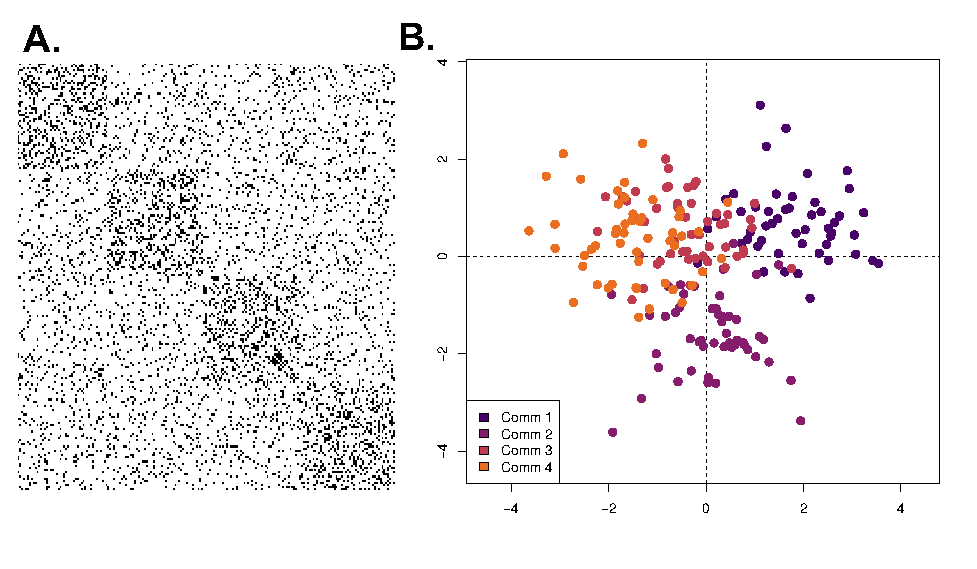
\includegraphics[width=0.5\textwidth]{SyntheticFig.pdf}
\caption{{\bf Synthetic Experiments.} NMI kmeans=0.68, NMI SBM=0.65, NMI attributeSBM=0.83}
\end{center}
\end{figure}





%%%%%%%%%%%%%%%%%%%%%%%

\section{Using the fitted attributed SBM for link prediction and collaborative filtering}
One of the benefits of a generative network model is that it can be applied to prediction tasks. Most notably, in the absence of one source of information about a node (connectivity or attributes), the model can be used to predict the complementary information source (attributes or connectivity, respectively). By fitting an attributed SBM, we found that obtain successful performance in two fundamental network prediction tasks, link prediction and collaborative filtering. 

In the link prediction problem, when given two node stubs, the objective is to determine whether a link exists between them. Since we are modeling connectivity with a stochastic block model, we can predict links using the learned parameters.  In particular, we highlight how this task can be performed using just the attribute information of the node stubs of interest. In the experiments to follow, we compare to 3 commonly-used link prediction methods. In all of these methods, a score is computed for all pairs of edge candidates and ultimately the top $x$ set of edges with highest weights are kept (where $x$ is some user-defined parameter). Let $m$ and $n$ be a pair of nodes and $\Gamma(m)$ denote the set of neighbors for a node $m$. Then, under the following 3 link prediction methods, we can calculate the score of the potential link as, $\text{Score}(m,n)$

{\bf Jaccard}: $\text{Score}(m,n)= \frac{\Gamma(m) \cap \Gamma(n)}{\Gamma(m)\cup \Gamma(n)}$

{\bf Adamic Adar}: $\text{Score}(m,n)=\sum_{c \in \Gamme(m) \cap \Gamma(n)}\frac{1}{\log |\Gamma(c)|}$

{\bf Preferential Attachment}: $\text{Score}(m,n}=|\Gamma(m)|\times |\Gamma(n)|$\\

Conversely, the collaborative filtering problem seeks to predict a node's attributes based on its similarity to its neighbors. For some node of interest, we can use our fitted attributed SBM model to predict a node's attributes, given only the information about its connectivity. Formally, for node $i$, we seek to predict ${\bf x}_{i}$. In the following experiments, we compare our results to two common collaborative filtering approaches. Let $\mathcal{N}^{k}(m)$ be the set of $k$-nearest neighbors in the network for node $m$. Let $\hat{{\bf x}_{i}}$ be the predicted attribute vector for node $i$ and $s_{ij}$ be a similarity measure between nodes $i$ and $j$. 

{\bf Neighborhood Avg}: $\hat{{\bf x}_{i}}= \frac{1}{|\mathcal{N}^{k}(i)|}\sum_{j \in \mathcal{N}^{k}(i)} {\bf x}_{j}$

{\bf Weighted Neighborhood Avg}: $\hat{{\bf x}_{i}}=\frac{1}{\sum_{j in \mathcal{N}^{k}(i)}s_{ij}}\sum_{j \in \mathcal{N}^{k}(i)}s_{ij}{\bf x}_{j}

We show results for these two tasks in two different biological network examples in section X. In particular, the experiments were designed in the following ways.

\subsection{Link Prediction Experiments}
 For our link prediction (figures x and y), we first choose 25 pairs of nodes that have an edge in the network and 25 pairs that do not. We then test each of these 50 edges in a leave one out manner. That is, for each of the 50 edges, we fit the attributed SBM to the network with the two stubs of the edge left out. We then use the nearest neighbor in attrivute space of each stub  as the the input to each of the 3 baseline community detection methods (Jaccard, Adamic Adar, and Preferential Attatchment). To use our attributed SBM in this link prediction task, we also consider the most commonly observed community among the 3 nearest neighbors for the stubs of the edge of interest. Again, using the nearest neighbors (denote $n$ and $m$ of the stubs, then we define the link prediction score for the edge as $\theta_{z_{n},z_{m}}$, or the probability that an edge exists between nodes $n$ and $m$ according to the fitted model. 

\subsection{Collaborative Filtering Experiments}
In collaborative filtering experiments, the objective is to predict the vector of attributes for each node. In our experiments, we used leave-one-out validation to predict the attribute vector for each node. That is, for each node in the network, we created a single node test set. The training set, was then the rest of the network with the node to predict removed. For this single test set node, we identified neighbors it connects to in only connectivity space within the training set. For standard collaborative filtering approaches (Neighborhood average and weighted neighborhood average), the predicted attribute for the test set node is then the specified averaging of the neighbors. To use our model for this task, we first fit the attributed SBM model to the training set. Similar to the standard link prediction approaches, we identify the nearest neighbors for our test node in connectivity space within the training set. We then predict the community membership of our test node to be the most-frequently observed community among its neighbors. Using this community assignment, $c$, we then predict the attribute vector for our test node to be ${\bf \mu}_{c}$, or the mean vector that was learned to describe community $c$. 



%%%%%%%%%%%%%%%%%%%%%%%%%%%%%%%%%%%

\section{Applications in Biological Networks}
While the motivation for the development of this method was not motivated by problems in biological data, we evaluate the potential to combine similarity or relational information between a set of entities, whether that be proteins, or biological samples, and experimental data and metadata. Our application of this model to biological problems provides a framework to predict attribute or connectivity information about a new observation.  Note that we do not intend to suggest any new biological insights, but rather that we can combine two sources of information for prediction tasks and alternative definitions of what constitutes a community in the data. 
\subsection{Microbiome Subject Similarity Results}

{\bf Motivation}

In the analysis of biological data, it is often useful to cluster subjects based on a set of their measure biological features and to then determine what makes each of the subgroups different. One type of biological data gaining much attention in recent years is metagenomic sequencing data, used to profile the composition of a microbiome. We refer to this as the 'metagenomic profile' and each feature is a count for each bacterial species, also known as operational taxonomic unit (OTU). In their paper (Ref. ), the authors conducted a study among subjects across a variety of ethnicities, body mass index (BMI) classifications, and age groups. Additionally, each subject has a count of 130 different bacterial species, obtained through sequencing. 

{\bf Pre-Processing}
We extracted a subset of the subjects being from Eastern Europe,Southern Europe ,Scandinavia, and the United States and constructed a between-subject similarity network between only individuals who had a BMI measurement. This resulted in a network of 121 nodes, where each edge is the pearson correlation between their microbial compositions. We then removed all edges in the network with weight (correlation) <0.7. 

{\bf Constructing Node Attributes}
We clustered samples (nodes) in this network using the Louvain community detection method into one of six clusters. We then built a random forest model to predict each sample's cluster assignment according to their metagenomic profiles. The attribute for each node was then the probability distribution of belonging to each of the 6 clusters of samples. This example highlights a novel way to combine two sources of information, between subject similarity and extra knowledge about the group memberships of the subjects. In figure 3A-B, we plot this subject similarity network and color the nodes by their community assignments using the classic and attributes stochastic block models, respectively. We also computed the normalized mutual information (NMI) between the node-to-community assignments identified from the partition under the louvain algorithm with the results obtained fitting the class and attributed SBM. Since the attributes of the nodes were the probability of belonging to each of the clusters identified under the Louvain algorithm partition, it was expected to observe a higher similarity between the Louvain partition with the attributed SBM partition than witth the SBM partition. This is exactly what we observed, with 0.78 being the NMI between the louvain algorithm partition and the classic SBM. Using the attributed SBM, we observed an NMI of 0.94 with the Louvain algorithm partition. 

\begin{figure}
\begin{center}
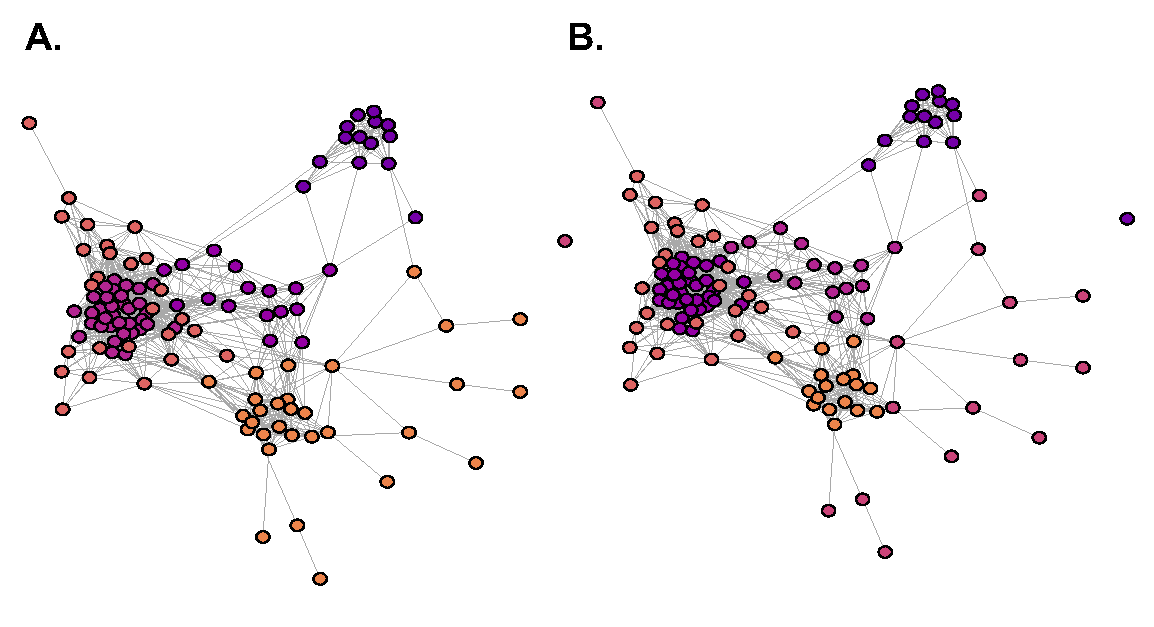
\includegraphics[width=0.5\textwidth]{MicrobiomeNet.pdf}
\caption{{\bf Visualization of fitting attributed model to microbiome subject similarity network:} Nodes are colored by one of 5 community assignments as predicted with the attributed SBM.}
\end{center}
\end{figure}

{\bf Microbiome Link Prediction}
In figure 4a-b we show the results for the link prediction in the sample similarity network. To perform link prediction, we selected 25 pairs of nodes (i.e. edge stubs) from our 121-node subject network. In our prediction task , we sought to model the ability to use only the attribute information and our fitted model to predict whether there was a link. Repeating this experiment 25 times, we obtained a distribution of area under the curve (AUC) values in figure 4A. and plotted the ROC curves corresponding to the experiment closest to the median for all link prediction methods. 
\begin{figure}
\begin{center}
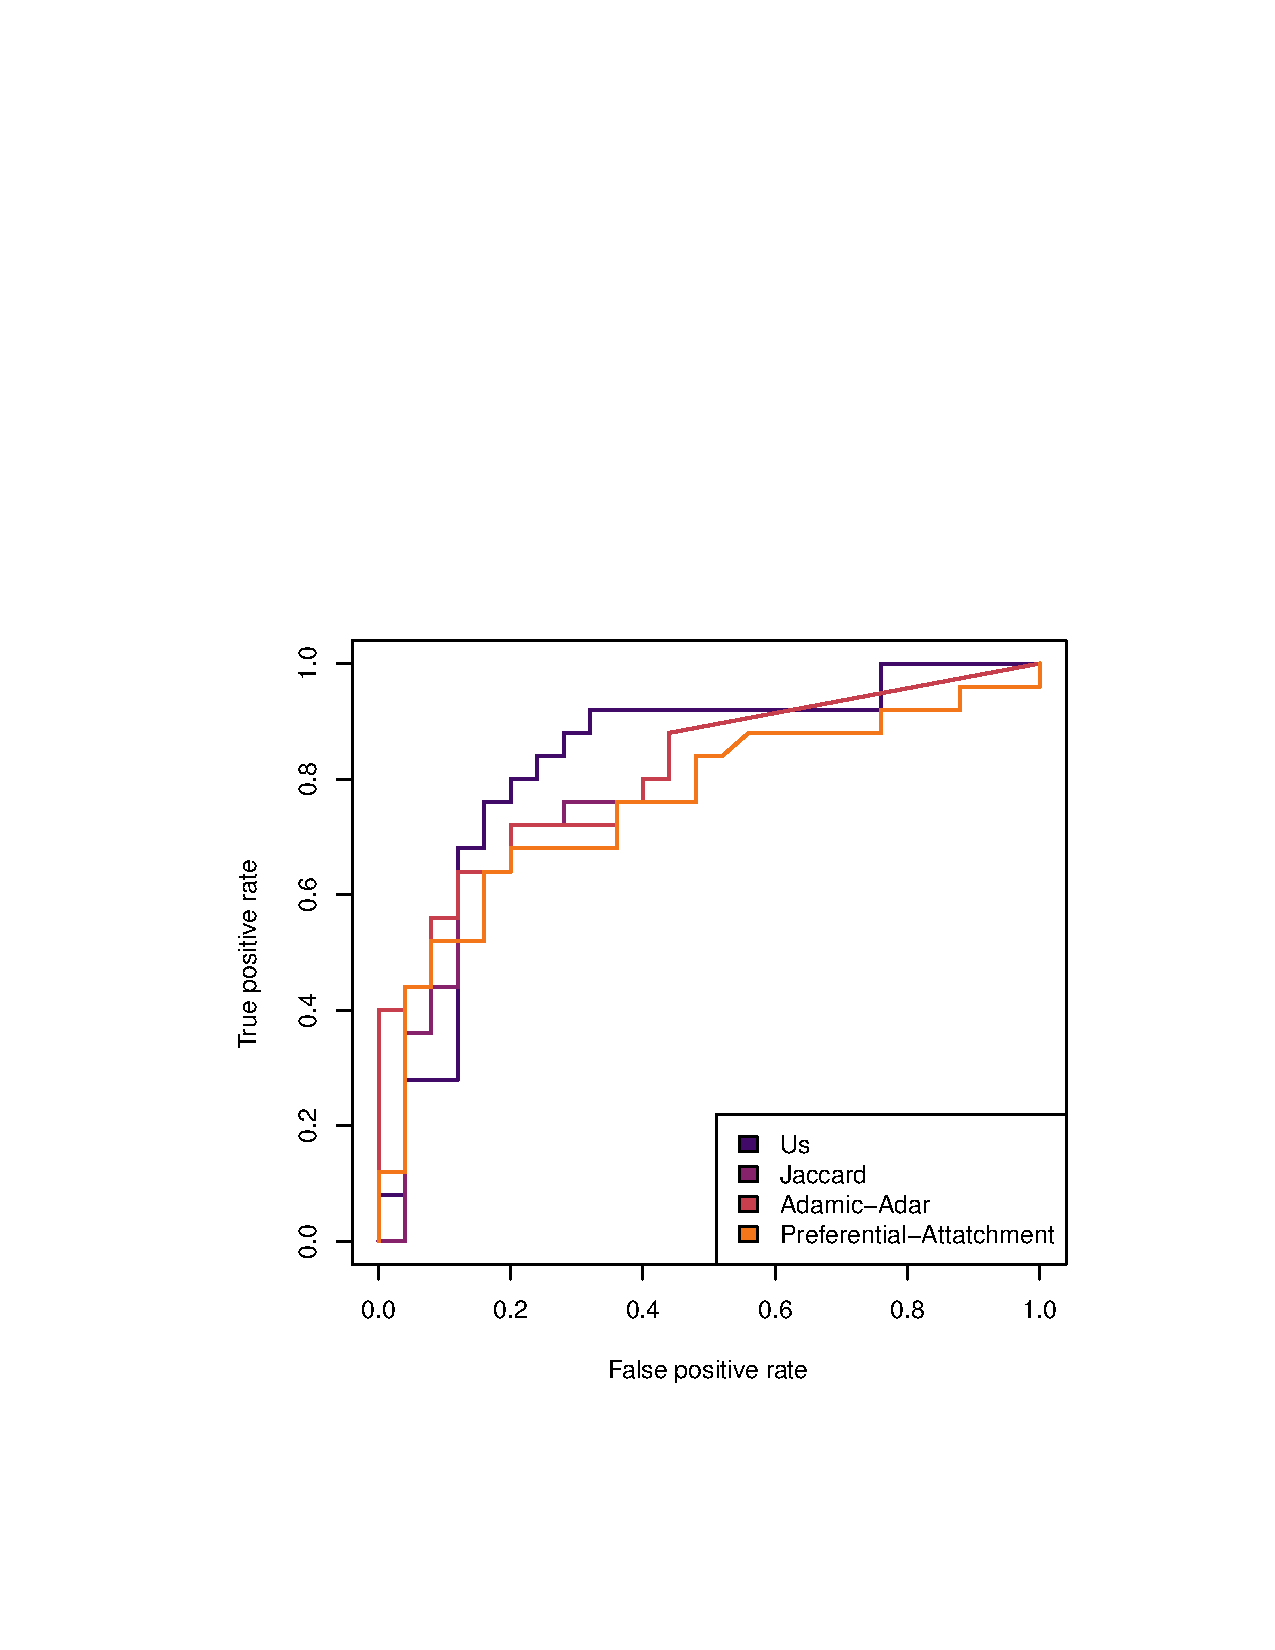
\includegraphics[width=0.4\textwidth]{Microbiome_LinkPred.pdf}
\caption{{\bf Link Prediction on the microbiome subject similarity matrix:}}
\end{center}
\end{figure}

{\bf Microbiome Collaborative Filtering}
Figure X shows the results for the collaborative filtering task on the subject microbiome network
\begin{figure}[h!]
\begin{center}
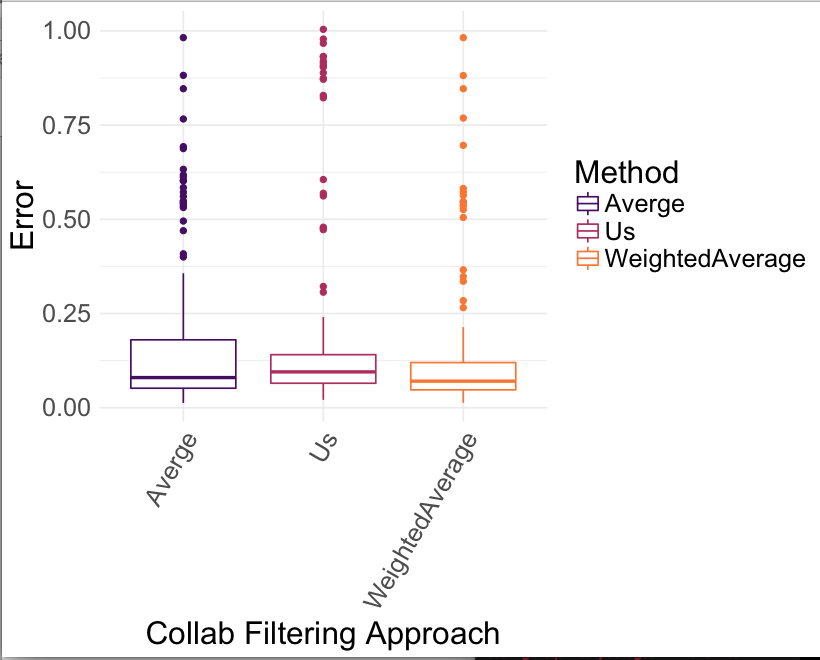
\includegraphics[width=0.4\textwidth]{CollabFilteringMicrobiome}
\caption{{\bf Collaborative Filtering Accuracy}: For each of the 121 nodes, we fit a model to the remaining 120 node network and given the node's closest network neighbors try to compute its attribute value. Error is the 2-norm between true and predicted attributes. }
\end{center}
\end{figure}

Here, we sought to predict the 6 dimensional attribute vector for each node. 

sahfkahfkjh insert more text

\subsection{Protein Interaction Network Results}
We also apply our attributed SBM approach to the protein interaction network presented in \cite{bonacci2014}. This network represents interactions between proteins, predicted from the literature. Associated with each each node (protein), is a vector of experimentally observed modifications resulting from the exposure of cancer cells to a chemotherapeutic drug. Proteins were able to undergo six possible modifications. While communities in this network should reflect functional relatedness among proteins, we also expect that members of a community should share similarities in the observed modification type. 

\begin{figure}[h!]
\begin{center}
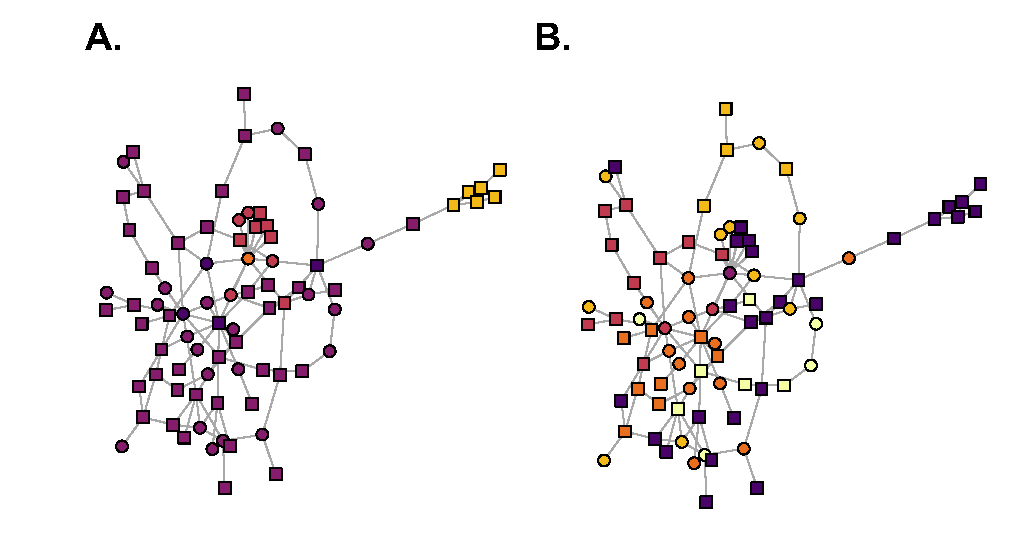
\includegraphics[width=0.5\textwidth]{ProteinNet.pdf}
\caption{{\bf Protein interaction network}}
\end{center}
\end{figure}

{\bf Data Pre-Processing: } We downloaded the network data and the modification information from the supplement of \cite{bonacci2014}. 

{\bf Constructing Node Attributes:}
For each node, we constructed its attributes vector as a vector of length 6, where each entry is a binary indicator for which of the 6 modifications was experimentally observed. 

Figure 6A-B show the results of fitting a classic SBM and attributed SBM, respectively.  The 6 possible modifications exist for 3 biological processes that can either increase or decrease. The node shape reflects whether the modification for a node was an increase (square) or decrease (circle). Nodes are colored by their assignment into 1 of x communities. (mention something about  the intuition behind the color groupings).

\begin{figure}[ht!]
\begin{center}
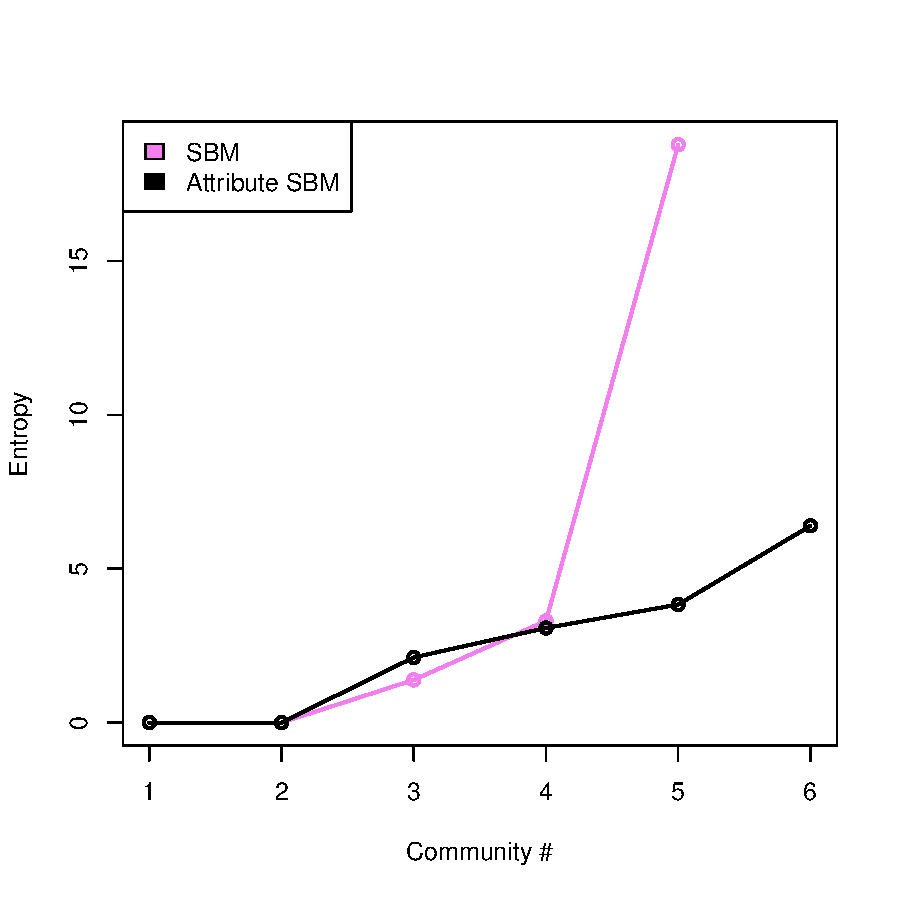
\includegraphics[width=0.45\textwidth]{EntropyCalc.pdf}
\caption{{\bf Community Entropies}}
\end{center}
\end{figure}

Next, we studied the entropies of these binary node classifications in each of the communities according to the regular and attributed SBM partitions. The hypothesis was that using the attributed SBM, we should have lower entropy of these two labels within communities because the attribute component of the model should assist in creating communities that are not only spatially relevant but also agree in attributes. 

{\bf Link Prediction in the Protein interaction network}
\begin{figure}[ht!]
\begin{center}
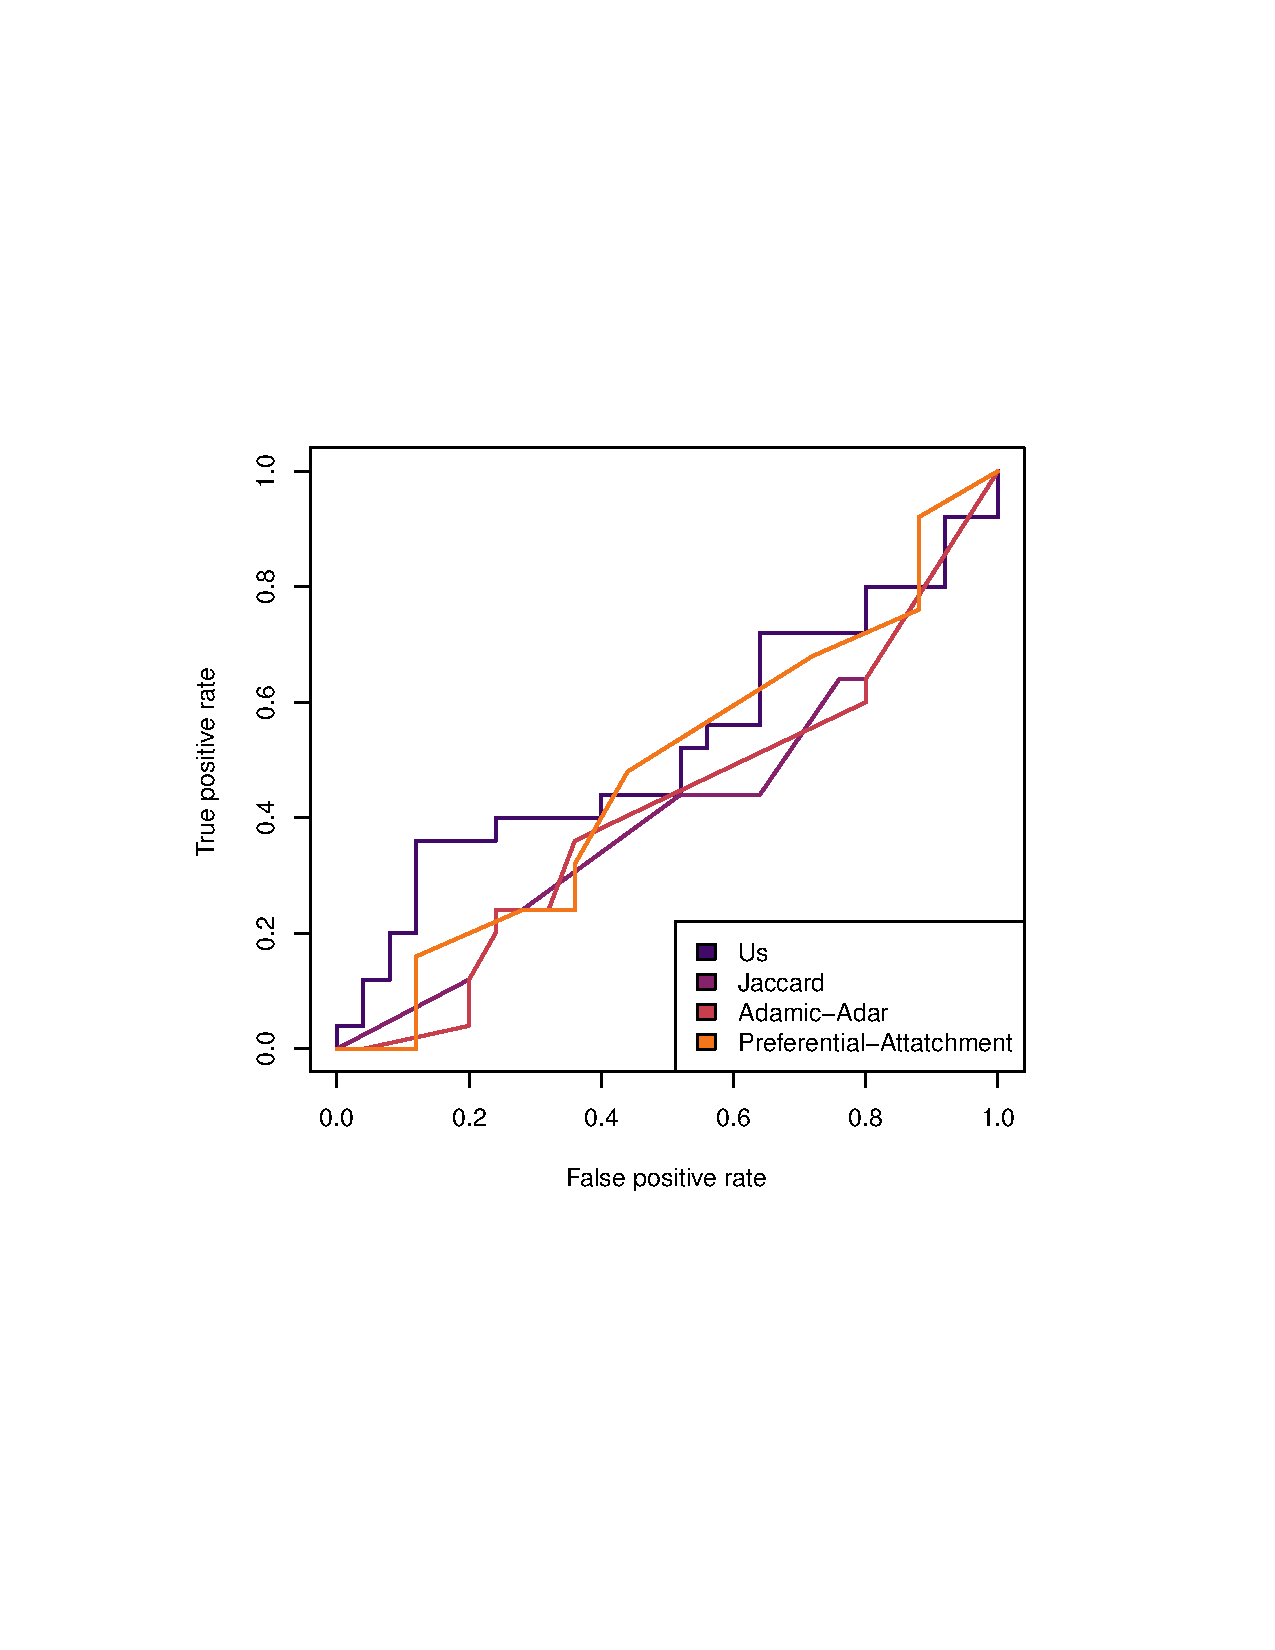
\includegraphics[width=0.4\textwidth]{Protein_LinkPred}
\caption{{\bf Community Entropies}}
\end{center}
\end{figure}


\section{Discussion}
Detectability problems



%\section{Segmentation Results}
%As an application of our method, we performed network-based image segmentation, where attributes were the 3-dimensional RGB color vectors and the adjacency matrix encoded sufficient \rk{what does sufficient mean?} spatial proximity. In this context, communities should correspond to objects or backgrounds/textures in the image. 
%
%\subsection{Image Pre-Processing}
%To perform network-based segmentation, we first created a super-pixel representation of an image  using SLIC \cite{SLIC}. That is, we took the original $391 \times 625$ (\rk{probably remove the exact dimensions)} matrix of pixels and aggregated homogeneous sets of pixels into a smaller set of super-pixels. We \rk{parametrized} SLIC to break the image into $\approx$~200 super-pixels, \rk{yet the algorithm sometimes produces} slightly less super-pixel. Next, for each super pixel, we computed its representative RGB vector, $\mathcal{C}$, as the mean of the RGB values, ${\bf c}=[R,G,B]$ of the original pixels (p) comprising the super-pixel. In other words, for super-pixel $S_{i}$, we can compute ${\mathcal C}_{i}$ as,
%\begin{equation}
%\mathcal{C}_{i}=\text{mean}({\bf c}_{p}), p \in S_{i}
%\end{equation}
%Since, we sought for the network of super pixels to reflect their spatial proximity, we computed the coordinate, ${\mathcal P}_{i}$ of super pixel $S_{i}$ as the median of the $x$ and $y$ coordinates $({\bf p}=[x,y])$ in the original grid of pixels. Then the \emph{coordinate} of super pixel ${\mathcal S}_{i}$ can be computed as,
%\begin{equation}
%\mathcal{P}_{i}=\text{median}({\bf p}_{p}),~p \in {\mathcal S}_{i}\enspace.
%\end{equation}
%Finally, the network was constructed by creating nearest neighbor graph. That is, for each super pixel, $\mathcal{S}_{i}$ we found its ${\mathcal N}$ nearest neighbors. So for $b \in \mathcal{N}_{i}$ we let $a_{\mathcal{S}_{i},b}=1$. Since the networks are undirected, we also enforced symmetry in ${\bf A}$. An example network from an image is shown in figure 3. 
%\begin{figure}
%\begin{center}
%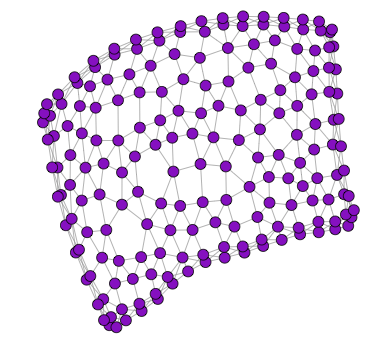
\includegraphics[scale=0.3]{TestGraph.png}
%\caption{{\bf Network of super pixels}. After aggregating the original $391 \times 625$ matrix of pixels into a super pixel representation, a network can be constructed to encode pairwise spatial proximity between super pixels. Each super pixel is connected with its ${\mathcal N}$ nearest spatial neighbors. }
%\end{center}
%\end{figure}
%\subsection{Segmentation Results}
%The segmentation results for 3 images (elephant, bird, and strawberry) from the Santner dataset \cite{Santner} are shown in figure 4. The top row of figure 4 shows the initial 3 images that we sought to segment. 
%\begin{figure}
%\begin{center}
%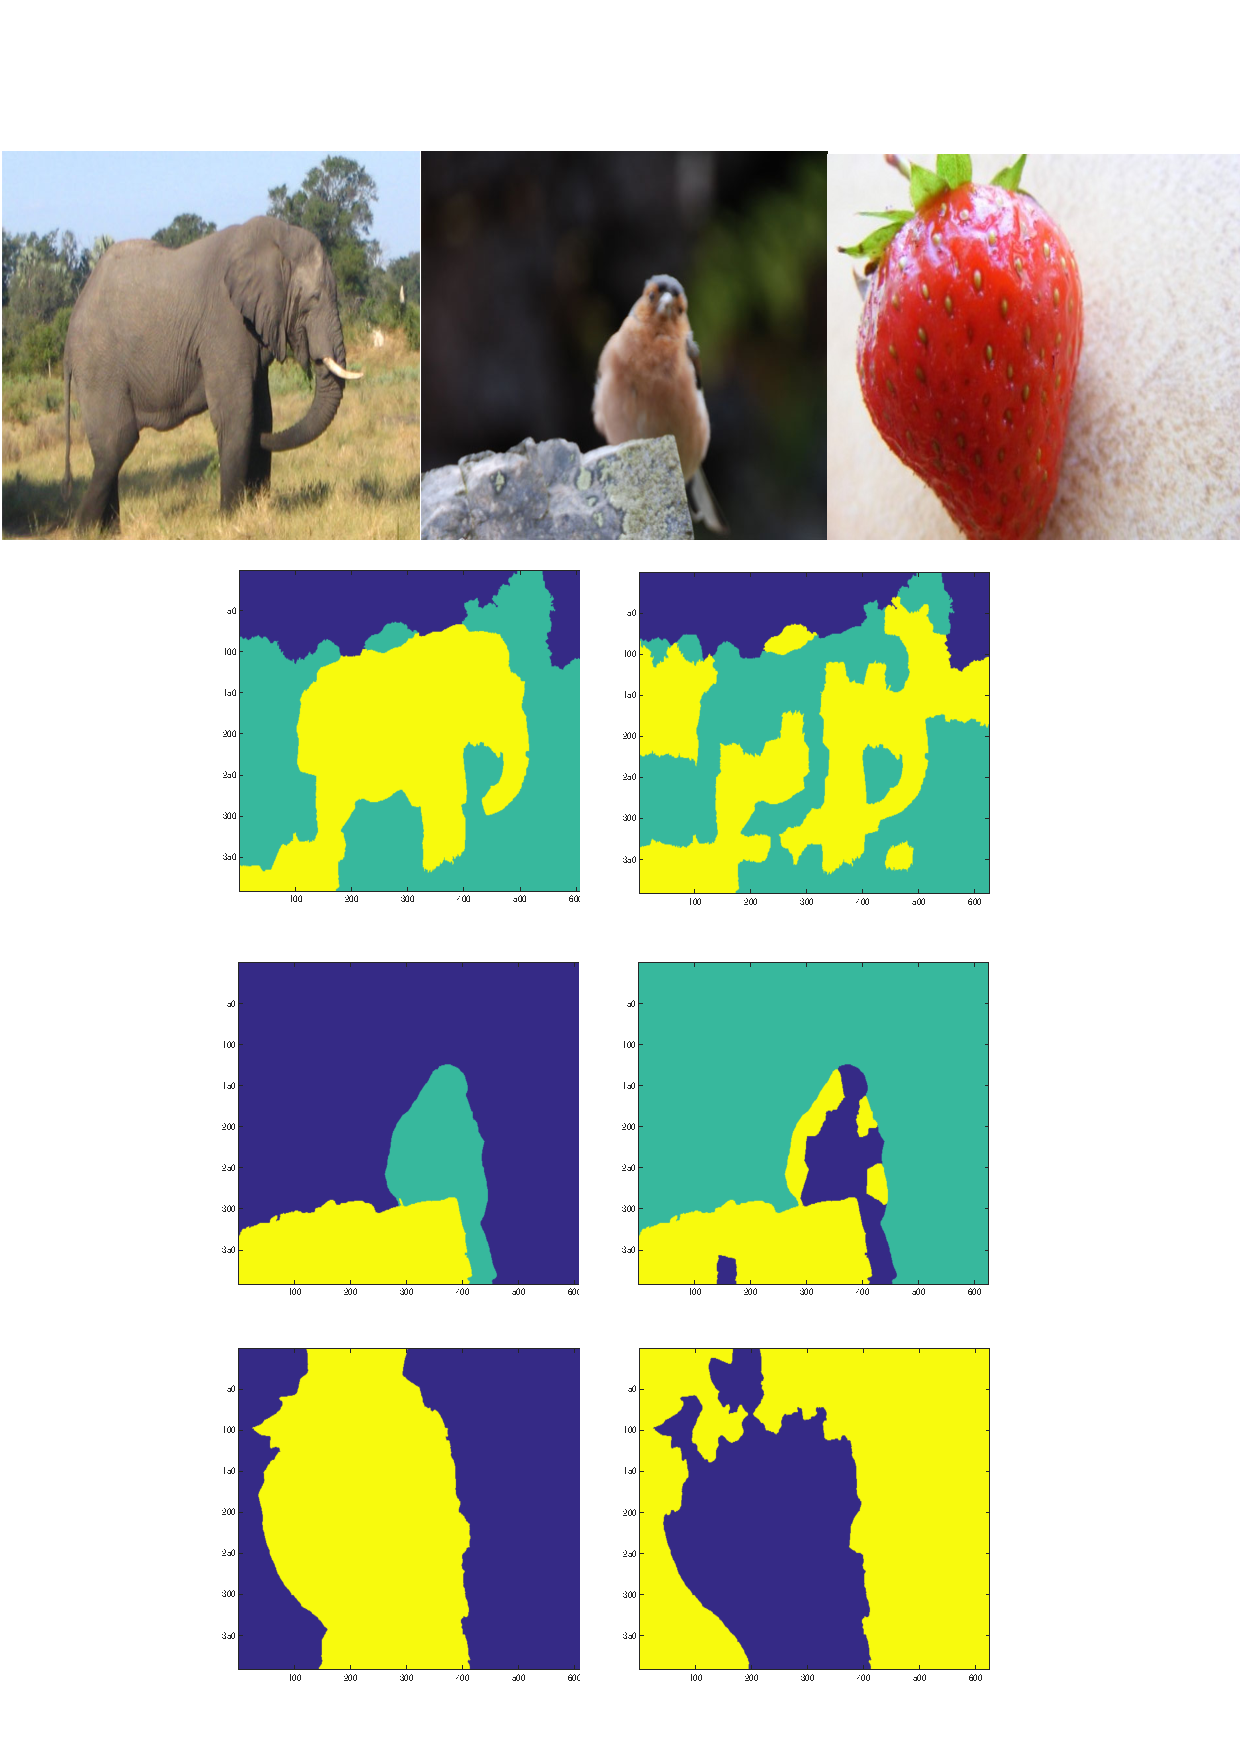
\includegraphics[scale=0.4]{segmentation.pdf}
%\caption{{\bf Example segmentation results}. Three images, elephant, bird, and strawberry were segmented according to our method (left column) as well as a baseline approach of concatenating adjacency matrix and attribute information (right column). Each image is first broken up into super pixels and a network is constructed between each super pixel and its ${\mathcal N}$ nearest neighbors, as defined by spatial distance.}
%\end{center}
%\end{figure}
%To compare our approach to a baseline method to integrate connectivity and attribute information, we concatenated these two sources of information into a single feature vector for each node and performed $k$-means clustering. In figure 4, the results of our method on each of the 3 images are shown in the left column, while those of the baseline clustering method are shown in the right. To quantitatively evaluate the accuracy of each segmentation result, we computed the dice score between our segmentation result and a human-labeled result from \cite{Santner}. These results are shown in table 2, where we also report the number of neighbors (${\mathcal N}$) used to construct the network of super pixels. In this table, Dice (us) refers to the dice score with our method, while Dice (baseline) gives the dice score for the clustering result with the concatenated feature vector. 
%
%\begin{table}
%\begin{center}
%\caption{ Segmentation results according to \emph{ground-truth} given by \cite{Santner}. The \emph{'Neighbors'} column reports how many neighbors were used to construct the network of 
%super-pixels 
%in a particular image. \emph{'Dice (us)'} gives the dice score for our method and 
%\emph{'Dice (baseline)'} gives the dice score for the baseline approach.}
%\begin{tabular}{ |c|c|c|c| } 
%\hline
%Image & Neighbors & Dice (us) & Dice (baseline)\\
%\hline
%elphant		& 10 & {\bf .4687} & .460	\\
%bird 		&  4 & {\bf .6187} & .2454 	\\
%strawberry 	&  7 & {\bf .9233} & .1346  \\
%\hline
%\end{tabular}
%\end{center}
%\end{table}


\section{Discussion}
To be filled in. 

%
% The following two commands are all you need in the
% initial runs of your .tex file to
% produce the bibliography for the citations in your paper.
\bibliographystyle{abbrv}
\bibliography{sigproc}  % sigproc.bib is the name of the Bibliography in this case
% You must have a proper ".bib" file
%  and remember to run:
% latex bibtex latex latex
% to resolve all references
%
% ACM needs 'a single self-contained file'!
%
%APPENDICES are optional
%\balancecolumns


%\balancecolumns % GM June 2007
% That's all folks!
\end{document}



